\begin{pro}
  Solve Poisson equation on the unit square.
\end{pro}
\begin{sol}
  We take the solution to be
  \begin{displaymath}
    u(x, y) = (x^2 - x^4)(y^4 - y^2),
  \end{displaymath}
  and therefore the right-hand side is given by
  \begin{displaymath}
    f(x, y) = 2\left[(1-6x^2)y^2(1-y^2)+(1-6y^2)x^2(1-x^2)\right].
  \end{displaymath}
  Modify the given code,
  and we obtain the following numerical result.
  Note that the convergence rate is obtained by the formula
  \begin{displaymath}
    p \approx
    \frac{\log(\|\mathbf{e}_h\|_{\infty}) - \log(\|\mathbf{e}_{2h}\|_{\infty})}{\log
    2}.
  \end{displaymath}
  \begin{figure}[H]
  \centering
  \subfigure[$N = 10$]{
    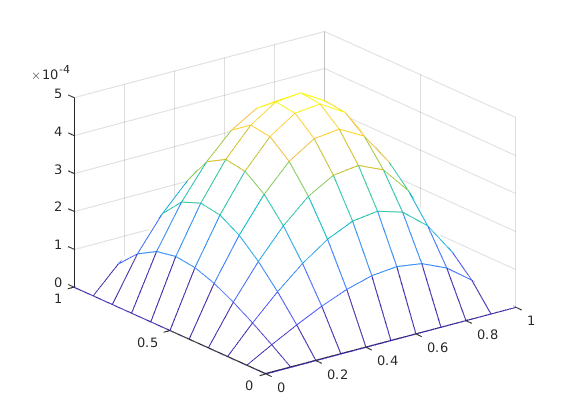
\includegraphics[width=0.235\linewidth]{png/poissonN10}
  }
  \hfill
  \subfigure[$N = 20$]{
    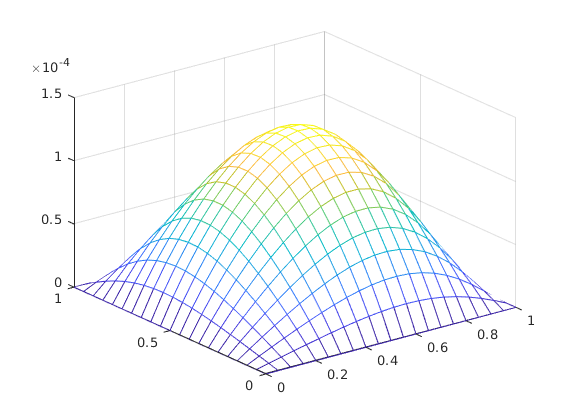
\includegraphics[width=0.235\linewidth]{png/poissonN20}
  }
  \hfill
  \subfigure[$N = 40$]{
    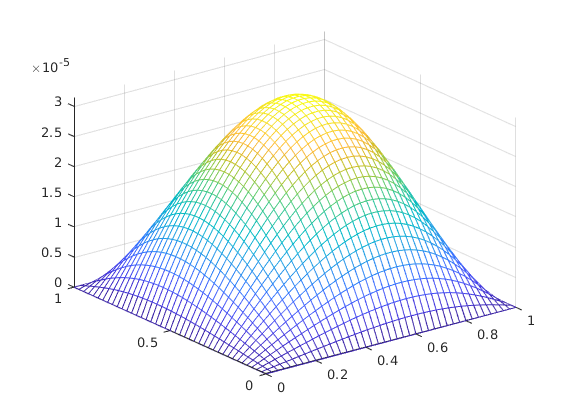
\includegraphics[width=0.305\linewidth]{png/poissonN40}
  }
  \hfill
  \subfigure[$N = 80$]{
    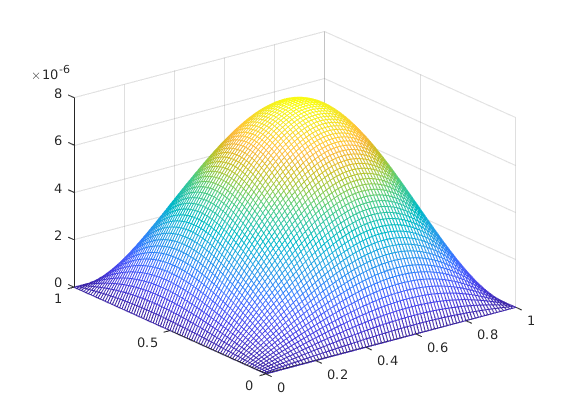
\includegraphics[width=0.305\linewidth]{png/poissonN80}
  }
  \hfill
  \subfigure[$N = 160$]{
    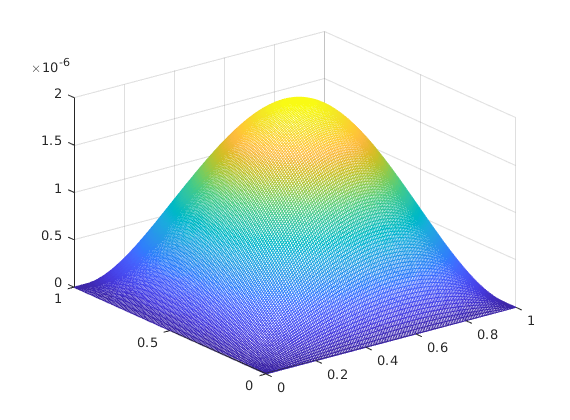
\includegraphics[width=0.305\linewidth]{png/poissonN160}
  }
  \hfill
  \subfigure[$N = 320$]{
    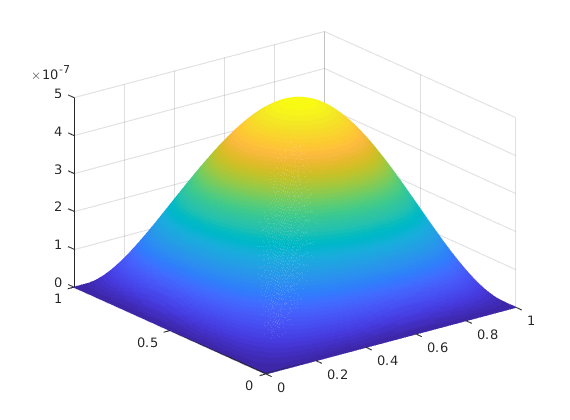
\includegraphics[width=0.305\linewidth]{png/poissonN320}
  }
  \hfill
  \subfigure[$N = 640$]{
    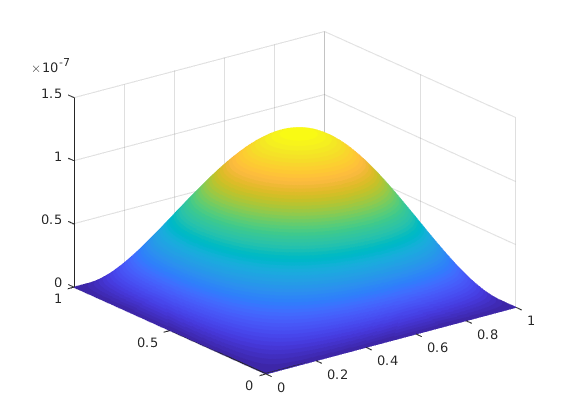
\includegraphics[width=0.305\linewidth]{png/poissonN640}
  }
  \hfill
  \subfigure[$N = 1280$]{
    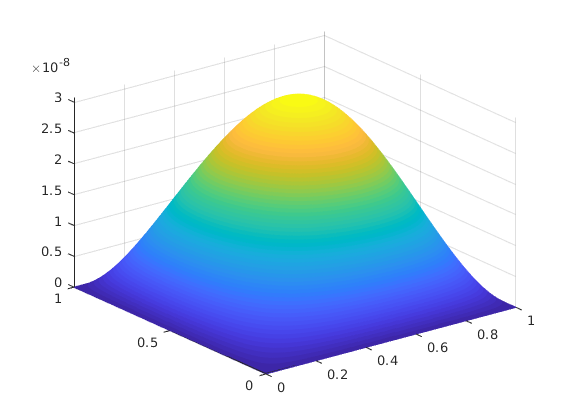
\includegraphics[width=0.305\linewidth]{png/poissonN1280}
  }
\end{figure}
\begin{figure}[H]
  \centering
\begin{tabular}{c|c|c}
  \centering
  $n$ & $\|\bm{e}^h\|_{\infty}$ & convergence rate
  \\ \hline
  10 & 4.99e-4 &
  \\
  20 & 1.26e-4 & 2.00
  \\
  40& 3.14e-5 & 2.00
  \\
  80 & 7.87e-6 & 2.00
  \\
  160 & 1.97e-6 & 2.00
  \\
  320 & 4.92e-7 & 2.00
  \\
  640 & 1.23e-7 & 2.00
  \\
  1280 & 3.07e-8 & 2.00
  \\ \hline
\end{tabular}
\end{figure}
Therefore,
the convergence rate of the proposed numerical scheme is $2$.
\end{sol}
%%% Local Variables:
%%% mode: latex
%%% TeX-master: "../hw5"
%%% End:
